%************************************************
\chapter{The \pkgname{ggplot2} package}\label{sec: ggplot2}
%************************************************
\texttt{install.packages(`ggplot2')}\\
\texttt{library(`ggplot2')}
\bigskip 

The package \texttt{ggplot2} allows to produce
graphs, plots and visual representations
constructing the aesthetics step by step,
incrementally adding different layers at the graphs. 
It is highly customisable due to this particular feature; 
we are going to show some of its main characteristics
in the below.

\section{General aesthetics}
Given a data frame, \texttt{ggplot} is invoked 
as \texttt{p <- ggplot(df)}, which corresponds to the
basic underlying plot object where we will construct
the rest of the layers upon, incrementally. Each 
additional layer is given by a set of points to 
be represented in the form of aesthetics that can be
plotted as points, lines, bars and so on and so forth.
Background colour is set by the option
\texttt{panel.background = element\_rect(fill = `\#002b36')}
within the \texttt{theme} aesthetics. General syntax is:
\begin{verbatim}
morley <- head(morley,20)
p <- ggplot(morley, aes(x=Run))
p <- p + theme(panel.grid.major = element_blank(), 
               panel.grid.minor = element_blank(),
               panel.background = element_rect(fill = '#002b36'),
               axis.line = element_line(colour = "black"),
               legend.text=element_text(size=16),
               legend.title=element_blank(),
               axis.title.x = element_text(vjust=0, size=16),
               axis.title.y = element_text(vjust=1, size=16),
               plot.title   = element_text(vjust=1.5, size=20)) 
p <- p + geom_line(aes(y=Speed), colour = '#268bd2' )
p <- p + geom_point(aes(y=Speed), colour = '#cb4b16')
p <- p + scale_x_discrete(breaks = morley$Run)
p <- p + labs(title = "Morley runs")
p <- p + labs(x = "Runs")
p <- p + labs(y = "Speed")
show(p)
\end{verbatim}

\section{Error bars}
If we want to add error bars we just have to add
\begin{verbatim}
error  <- 10*rnorm(20)
dodge  <- position_dodge(width=0.9)
p      <- p + geom_errorbar(aes(ymin= Speed - error, 
	        ymax = Speed + error), position = dodge,
            colour="blue", width=.1)
\end{verbatim}
\begin{figure}[htbp]
 \centering
 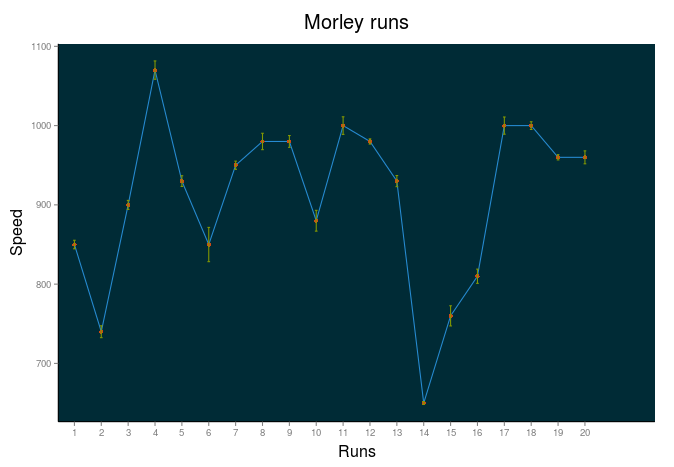
\includegraphics[scale=0.5]{images/error_bars}
 \caption*{Plot with error bars}
\end{figure}

\section{Barplots}
If, instead, we want to have a barplot thereof, just
replace \texttt{geom\_line} (\texttt{geom\_point} respectively)
with

\begin{verbatim}
p <- p + geom_bar(aes(y=Speed),stat='identity', width=.7,
         fill='#657b83', color= '#6c71c4')
\end{verbatim}
\begin{figure}[htbp]
 \centering
 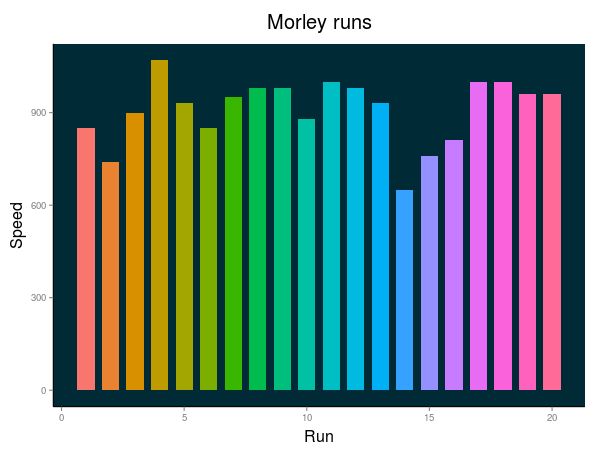
\includegraphics[scale=0.5]{images/barplot}
 \caption*{Barplot}
\end{figure}
                  
How about we unfold the bars in polar coordinates
instead?

\texttt{p <- p + coord\_polar()}

\begin{comment}
\begin{figure}[htbp]
 \centering
 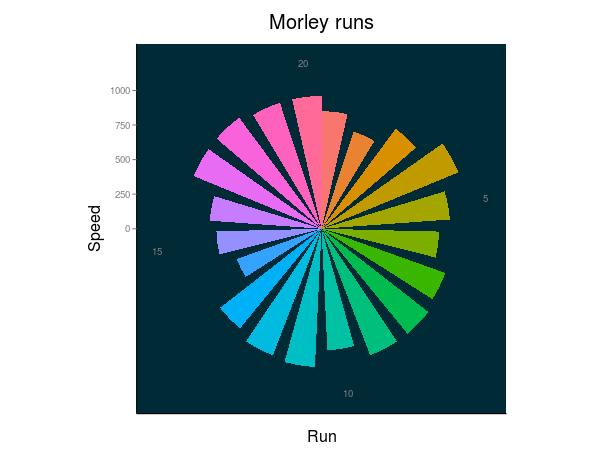
\includegraphics[scale=0.35]{images/polar}
 \caption*{Barplot in polar coordinates}
\end{figure}
\end{comment}

\section{Boxplots}
A boxplot is obtained as follows (\texttt{theme} is kept as before):
\begin{verbatim}
p <- ggplot(morley, aes(x=2, y=morley$Speed))
p <- p + geom_boxplot(outlier.colour = "blue", fill="grey85") 
p <- p + labs(title = "Morley speeds")
p <- p + labs(y = "Speed")
p <- p + labs(x = "")
show(p)
\end{verbatim}
where the values of the $x$ axis is irrelevant. Additional options
can be included with
\begin{verbatim}
p <- p + geom_boxplot(notch = TRUE) 
p <- p + geom_jitter() 
p <- p + geom_hline(aes(yintercept=mean(morley$Speed)), 
	 colour="sienna")
\end{verbatim}

\begin{figure}[htbp]
 \centering
 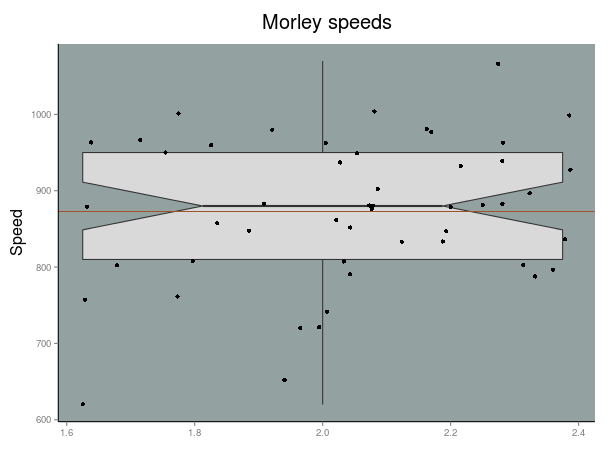
\includegraphics[scale = .50]{images/jitter}
 \caption*{Boxplot with jitters and notches}
\end{figure}

\section{Data grouped by}
Should we have data belonging to different 
groups, it would be convenient to represent
each one of them with different colours, lines
and bars. Here is how:
\begin{verbatim}
library(data.table)
iris   <- data.table(iris)
groups <- iris[, .(length = mean(Sepal.Length)), 
	      by = c("Species", "Sepal.Width")]

p <- ggplot(groups, aes(x=Sepal.Width, y=length, 
		   group = Species, colour= Species))
p <- p + theme(panel.grid.major = element_blank(), 
               panel.grid.minor = element_blank(),
               panel.background = element_rect(fill = '#002b36'),
               axis.line = element_line(colour = "black"),
               legend.text=element_text(size=16),
               legend.title=element_blank(),
               axis.title.x = element_text(vjust=0, size=16),
               axis.title.y = element_text(vjust=1, size=16),
               plot.title   = element_text(vjust=1.5, size=20)) 
p <- p + geom_point()
p <- p + geom_line() 
p <- p + scale_colour_discrete()
p <- p + labs(title = "Iris species")
p <- p + labs(x = "Sepal width")
p <- p + labs(y = "Sepal length")
show(p)      
\end{verbatim}
\begin{figure}[htbp]
 \centering
 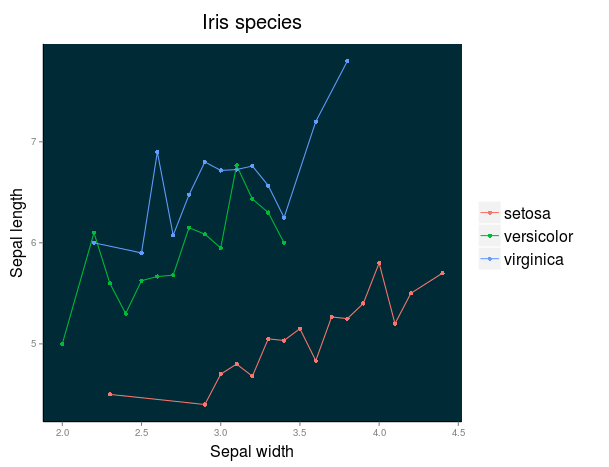
\includegraphics[scale = .65]{images/grouped_colours}
 \caption*{Data grouped by distinguished by colours}
\end{figure}

Equivalently with barplots
\begin{verbatim}
iris <- data.table(iris)
iris$Sepal.Width <- round(iris$Sepal.Width)
groups <- iris[, .(length = mean(Sepal.Length)), 
		  by = c("Species", "Sepal.Width")]


p <- ggplot(groups, aes(x=Sepal.Width, y=length))
p <- p + theme(panel.grid.major = element_blank(), 
               panel.grid.minor = element_blank(),
               panel.background = element_rect(fill = '#002b36'),
               axis.line = element_line(colour = "black"),
               legend.text=element_text(size=16),
               legend.title=element_blank(),
               axis.title.x = element_text(vjust=0, size=16),
               axis.title.y = element_text(vjust=1, size=16),
               plot.title   = element_text(vjust=1.5, size=20)) 
p <- p + geom_bar(aes(fill=Species), width = 0.8, 
                  position = "dodge", stat = "identity")
p <- p + scale_colour_discrete()
p <- p + labs(title = "Iris species")
p <- p + labs(x = "Sepal width")
p <- p + labs(y = "Sepal length")
show(p)
\end{verbatim}
\begin{figure}[htbp]
 \centering
 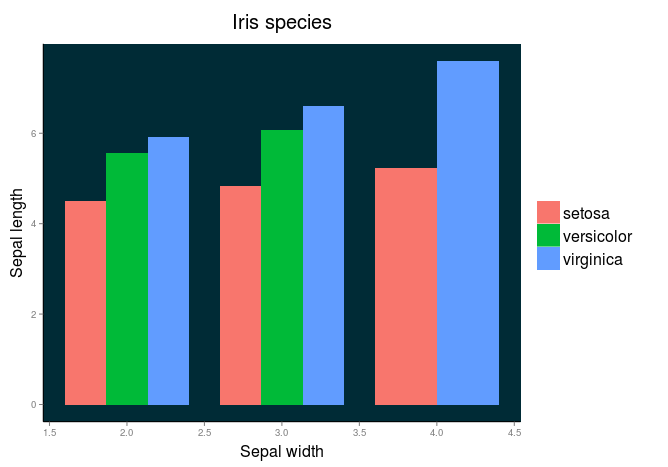
\includegraphics[scale = .5]{images/grouped_barplot}
 \caption*{Barplot of data grouped by}
\end{figure}

The option \texttt{position = "dodge"}
ensures that the bars lie by one other. Taking 
that off would make a stacked barplot instead.
Adding the option \texttt{faced\_grid} allows to move 
different groups to different windows of the graph
\texttt{p <- p + facet\_grid(Species \~ .)}
\begin{figure}[htbp]
 \centering
 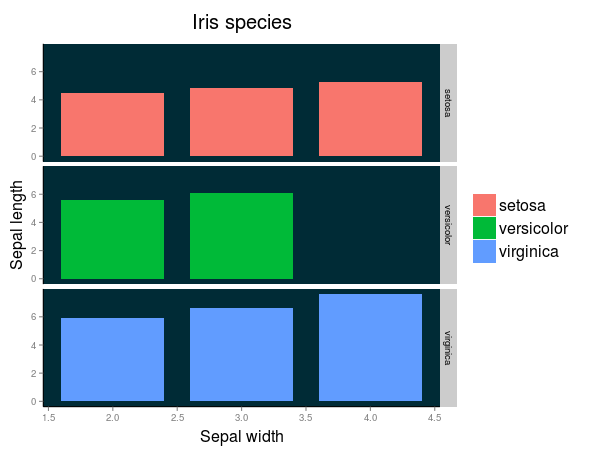
\includegraphics[scale=0.6]{images/facet_grid}
 \caption*{Barplots in different windows}
\end{figure}

\section{Plotting functions}
In order to plot several functions on
the same graph
\begin{verbatim}
p <- ggplot(data.frame(x = c(-5, 5)), aes(x))  
p <- p + stat_function(fun = dnorm, colour = "#2aa198")
p <- p + stat_function(fun = function(x) 2*dnorm(x^2-1), 
		      colour = "#268bd2")
p <- p + theme(panel.grid.major = element_blank(), 
               panel.grid.minor = element_blank(),
               panel.background = element_rect(fill = '#002b36'),
               axis.line = element_line(colour = "black"),
               legend.text=element_text(size=16),
               legend.title=element_blank(),
               axis.title.x = element_text(vjust=0, size=16),
               axis.title.y = element_text(vjust=1, size=16),
               plot.title   = element_text(vjust=1.5, size=20)) 
show(p)
\end{verbatim}
\begin{figure}[htbp]
 \centering
 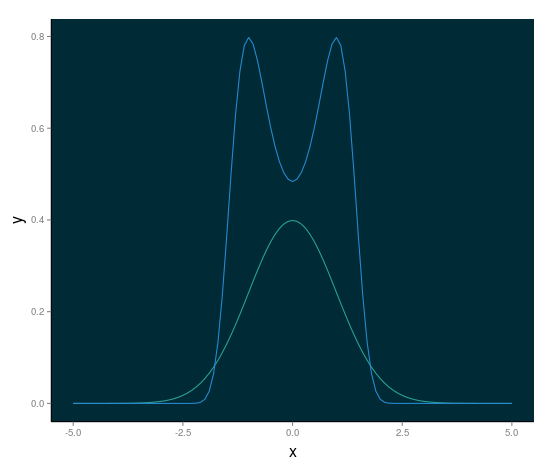
\includegraphics[scale = .45]{images/functions}
 \caption*{Plot of more than one function}
\end{figure}

\section{Histograms}
\texttt{geom\_histogram} does the job. The values 
have to nevertheless be made into a data table 
format, that has to be invoked as first argument
of \texttt{ggplot}
\begin{verbatim}
dt <- data.table(values = rlnorm(50))

p <- ggplot(dt, aes(x=values))
p <- p + theme(panel.grid.major = element_blank(), 
               panel.grid.minor = element_blank(),
               panel.background = element_rect(fill = '#002b36'),
               axis.line = element_line(colour = "black"),
               legend.text=element_text(size=16),
               legend.title=element_blank(),
               axis.title.x = element_text(vjust=0, size=16),
               axis.title.y = element_text(vjust=1, size=16),
               plot.title   = element_text(vjust=1.5, size=20)) 
p <- p + geom_histogram(aes(y=..density.., fill = ..density..), 
                        colour="#002b36", binwidth = 0.3)
p <- p + geom_density(color = "#657b83")
# the below is to manually set the gradient
# p <- p + scale_fill_gradient(low = "red", high = "green")
p <- p + labs(title = "Histogram of normal samples")
show(p) 
\end{verbatim}
\begin{figure}[htbp]
 \centering
 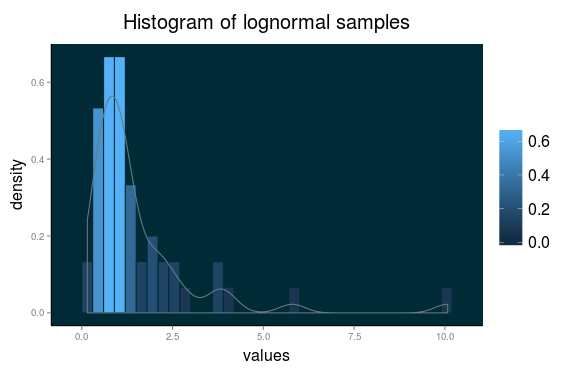
\includegraphics[scale = .45]{images/histogram}
 \caption*{Histogram}
\end{figure}

\section{Tiles}
\texttt{install.packages(scale)}\\
\texttt{library(scale)}
\bigskip 

A powerful visualisation method for many variables
at a time is provided by \texttt{geom\_tile}, where different
values of each variable are represented by different tiles
filled on gradient according to the value: the set 
of data must be molten first and then the variables values
have to be scaled between $\mathopen[0,1\mathclose]$ so 
that one can assign standard gradient fillings. The
example below clarifies the issue:
\begin{verbatim}
cars          <- data.table(mtcars)
cars$carnames <- rownames(mtcars)
cars.molten   <- melt(cars)

R: cars.molten <- data.table(cars.molten)
R: cars.molten[sample(.N,5)]

              carnames variable value
1:            Merc 230     qsec 22.90
2:         Honda Civic       am  1.00
3:           Merc 240D     drat  3.69
4: Lincoln Continental      mpg 10.40
5:          Merc 450SL       am  0.00
\end{verbatim}
We now make use of the \texttt{rescale} function
in the \texttt{scale} package as:
\begin{verbatim}
cars.molten <- ddply(cars.molten, .(variable), transform,
                rescale = rescale(value)) 
R: cars.molten <- data.table(cars.molten)
R: cars.molten[sample(.N,5)]

              carnames variable value   rescale
1:          Camaro Z28      mpg  13.3 0.1234043
2:          Merc 450SE      mpg  16.4 0.2553191
3:          Camaro Z28     disp 350.0 0.6956847
4: Lincoln Continental       hp 215.0 0.5759717
5:           Merc 280C     qsec  18.9 0.5238095

p <- ggplot(cars.molten, aes(x=variable, y = carnames, 
                                      fill = rescale))
p <- p + theme(panel.grid.major = element_blank(), 
               panel.grid.minor = element_blank(),
               panel.background = element_rect(fill 
                                            = '#002b36'),
               axis.line = element_line(colour = "black"),
               legend.text=element_text(size=16),
               legend.title=element_blank(),
               axis.title.x = element_text(vjust=0, 
                                     size=16),
               axis.title.y = element_text(vjust=1, size=16),
               plot.title   = element_text(vjust=1.5, size=20)) 
p <- p + geom_tile(colour = "#002b36")
p <- p + scale_fill_gradient(low = "steelblue", 
                             high = "#002b36")
p <- p + labs(x = "")
show(p)
\end{verbatim}
Tiled results are shown in the plot below, whit the 
row names arranged on the $y$ axis and the variables 
displayed horizontally instead.
\begin{figure}[htbp]
 \centering
 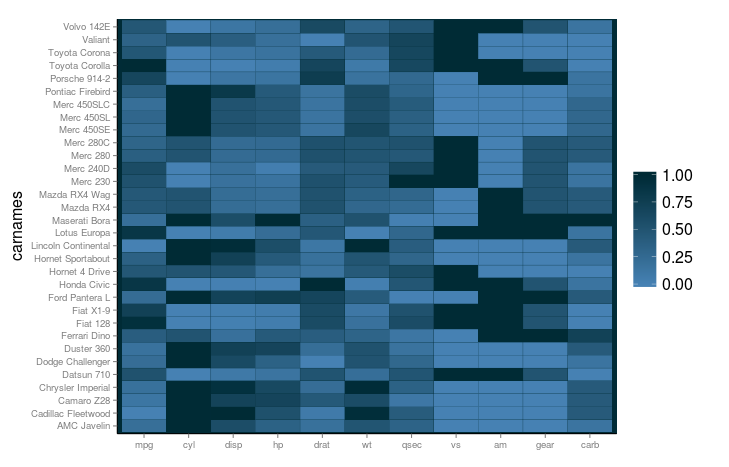
\includegraphics[scale=0.5]{images/tiles}
 \caption*{Tiled heatmap}
\end{figure}